\documentclass[conference]{IEEEtran}
\IEEEoverridecommandlockouts
% The preceding line is only needed to identify funding in the first footnote. If that is unneeded, please comment it out.
\usepackage{cite}
\usepackage{amsmath,amssymb,amsfonts}
\usepackage{algorithmic}
\usepackage{graphicx}
\graphicspath{{images/}}
\DeclareGraphicsExtensions{.pdf,.jpeg,.png}

\usepackage{textcomp}
\usepackage{xcolor}
\usepackage{url}

% For sub figures
\usepackage{subcaption}

% For interactive sharing
\usepackage{soul}
\newcommand{\hlc}[2][yellow]{ {\sethlcolor{#1} \hl{#2}} }
\newcommand{\sm}[1]{\hlc{#1}}
\newcommand{\smb}[1]{\hlc[green]{#1}}

\newcommand{\etal}{\textit{et al.}\xspace}
\newcommand{\idest}{\textit{i.e.}\xspace}
\newcommand{\eg}{\textit{e.g.}\xspace}
\newcommand{\aka}{\textit{a.k.a.}\xspace}
\newcommand{\tit}[1]{\textit{#1}}
\newcommand{\thi}[1]{\texttt{#1}}
\newcommand{\gra}[1]{\textbf{#1}}

\begin{document}

\title{LOFAR archive data processing for the mass*\\
{\footnotesize \textsuperscript{*}Note: Sub-titles are not captured in Xplore and
should not be used}
\thanks{Identify applicable funding agency here. If none, delete this.}
}

\author{\IEEEauthorblockN{1\textsuperscript{st} Given Name Surname}
\IEEEauthorblockA{\textit{Netherlands eScience Center}\\
Amsterdam, The Netherlands \\
G.Surname@esciencecenter.nl}
\and
\IEEEauthorblockN{2\textsuperscript{nd} Given Name Surname}
\IEEEauthorblockA{\textit{Netherlands eScience Center}\\
Amsterdam, The Netherlands \\
G.Surname@esciencecenter.nl}
\and
\IEEEauthorblockN{3\textsuperscript{rd} Given Name Surname}
\IEEEauthorblockA{\textit{Netherlands eScience Center}\\
Amsterdam, The Netherlands \\
G.Surname@esciencecenter.nl}
\and
\IEEEauthorblockN{4\textsuperscript{th} Given Name Surname}
\IEEEauthorblockA{\textit{dept. name of organization (of Aff.)} \\
\textit{name of organization (of Aff.)}\\
City, Country \\
email address}
\and
\IEEEauthorblockN{5\textsuperscript{th} Given Name Surname}
\IEEEauthorblockA{\textit{dept. name of organization (of Aff.)} \\
\textit{name of organization (of Aff.)}\\
City, Country \\
email address}
\and
\IEEEauthorblockN{6\textsuperscript{th} Given Name Surname}
\IEEEauthorblockA{\textit{dept. name of organization (of Aff.)} \\
\textit{name of organization (of Aff.)}\\
City, Country \\
email address}
}

\maketitle

\begin{abstract}
This document is a model and instructions for \LaTeX.
This and the IEEEtran.cls file define the components of your paper [title, text, heads, etc.]. *CRITICAL: Do Not Use Symbols, Special Characters, Footnotes, 
or Math in Paper Title or Abstract.
\end{abstract}

\begin{IEEEkeywords}
component, formatting, style, styling, insert
\end{IEEEkeywords}

\section{Introduction}
[…]

The LOFAR telescope is usually dubbed as ``software'' telescope, meaning it relies on software to reach its goals. This is visible in the operational design of the instrument as, before even being stored as data, the signals go through a computing system, the correlator, where they are processed (correlated) and then sent to the LTA as visibilities. These pre-processed data are seldom used directly by the astronomers. Instead, these data usually go through further processing for, for instance, radio frequency interference removal, calibration and finally imaging. The generated images are the inputs to most scientific enquiries.

    Each of above processing is complex and requires usually both domain and software knowledge in order to be used to generate useful output. This combined with the massive volume of the data makes the use of the LTA only possible to a select group of people. Furthermore, these challenges are exacerbated when one needs to process, not only one observation but as many as possible simultaneously as is the case for surveys. For this reason, researchers interested in surveys for instance, are building frameworks to make LOFAR observation processing easy, portable, scalable and generalisable\cite{mechev2017}.

One of the achievements of the above project is making the workflow processing possible on some clusters connected to the LTA with high-bandwidth network (SURFSara) and accelerating some of the processing steps by using parallel computing, which can be seen as vertical scalability. One of the aims the project didn’t reach yet is horizontal scalability. This is where the EU PROCESS\footnote{\url{https://process-project.eu}} project comes into play. Indeed, PROCESS is designed to tackle the extreme large data handling and processing challenges introduced by exascale applications such as surveys. The approach taken PROCESS is to build tools and services capable of supporting exascale use cases by federating computing infrastructures from both HPC and Cloud. It comes at no surprise, LOFAR surveys is one of five pilot applications in PROCESS which will bring horizontal scalability to above work by making it possible to run several processing workflows in parallel on several computing infrastructures.

One of the goals of PROCESS is to facilitate the use of the resulting platform by providing a user-friendly frontend that lets the user select both her datasets and workflows, launch the processing to the computing infrastructures and, finally, either directly or indirectly retrieve the results from the frontend. For the particular case of LOFAR data processing, such a tool already already exists, although it needs to be customised and extended. Indeed, as part of the EU EOSCpilot project\footnote{\url{https://eoscpilot.eu}}, an astronomer-friendly frontend to LOFAR LTA has been built.

\section{Background}
%\subsection{LOFAR software stack}
%\subsection{EOSC pilot for LOFAR}
%\subsection{Xenon-flow and CWL}
%\subsection{Containerisation and data services in PROCESS}

The use of the LOFAR telescope by the different key science projects (KSP) is based on the concept of pipeline. A pipeline is a chain structured as a directed acyclic graph (DAG) of processing steps, each step taking some inputs, performing some processing and generating some outputs. This pipeline framework is used to automate processing on computing facilities (at ASTRON). For instance, almost every KSP has its own pipeline.
% This concept is deeply entranched into the way the telescope data are used.
Writing a pipeline is quite complex and requires knowledge of the pipeline framework and programming skills. Because of this, a specific pipelines, called \thi{genericpipeline}, is offered for helping users design and execute their workflows without understanding the underlying pipeline system. Usually, there are enough predefined steps for the user to choose from, so that defining a pipeline with the \thi{genericpipeline} boils down to defining configuring a minimal set of program arguments. Steps and arguments are defined in a so-called parameter set (\thi{parset}) file which is the argument to the \thi{genericpipeline}.
Most astronomers use images as starting point for their analysis. The generation of those images goes through several steps, including pre-processing, calibration and actual imaging. One common tool used in this process is \thi{prefactor} which consists of various \tit{parsets} for the \thi{genericpipeline} that do the direction-independent (DI) calibration of LOFAR data. Originally intended to prepare the data for use by the direction-dependent (DD) calibration software \thi{factor} (thus, the name), \thi{prefactor} corrects for various instrumental and ionospheric effects on observations and makes them ready for other DD calibration software, such as \thi{killMS}, as well. It is essentially composed of two pipelines: the \tit{calibrator} pipeline processing the calibrator to derive the DI corrections and the \tit{target} pipeline transferring the DI corrections to the target and performing DI calibration on the target.

As part of the EOSCpilot, work has been done to make LOFAR data available to a broader audience for enabling groundbreaking scientific discoveries. To reach this goal, access to LOFAR is made according to FAIR principles and containerisation is used to make processing portable across EOSC infractures. Containerisation is a new of delivering software preinstalled in an isolated environment, bundled with all its dependencies. This makes software installation easy, as the user only needs the actual container once the container software is in place. Whatsmore in EOSCpilot, the common workflow language (CWL\footnote{\url{https://www.commonwl.org/v1.0/}}) is used to ensure data analysis workflows portability across systems. Concretely, the output of the EOSCpilot for LOFAR data is astronomer-friendly Web application where she can select an observation from LTA and a pipeline from the frontend, then launch the processing to the backend supported by EOSC infrastructures using CWL and Singularity\footnote{\url{https://www.sylabs.io}}. Unfortunately, we are using a remote execution framework which is not support by work within EOSCpilot. Yet, we use the frontend for data selection.

For the remote execution framework used in this work is the \thi{xenon-flow}\footnote{\url{https://github.com/xenon-middleware}} middleware which runs CWL workflows using \thi{xenon}\cite{jason_maassen_2015_35415}. Xenon is a middleware abstraction library providing a simple programming interface to many remote compute and storage resources and hiding the complex protocol and tool specific details from the application. This allows the application to switch without changing the code. Xenon is based on a few fundamental concepts, including credentials, file system, scheduler and job. Credentials contain functionality for gaining access to resources, file systems for file management and schedulers create and manage jobs usually though a workload management system.

\section{Implementation and Results}
The Web application (LTACAT) is an Angular application inherited from FRBCAT project. That application customised to fit LOFAR LTA needs: the frontend stayed almost identical, but showing information about observation, instead of fast radio bursts (FRBs); the backend is rewritten to use the LTA database view, which lets the application seamlessly access the observational archived data. A Django REST API project is then added to the framework allowing users to develop pipeline and run them from the Web application. The application comes bundled with a pre-defined pipeline, \thi{LGPPP\_LOFAR\_pipeline}.

 A pipeline template and a procedure are provided for the definition of new pipelines as a Django application within the project. The procedure consists roughly in implementing a \tit{run} function, modifying and renaming a few files in the template Getting a new pipeline added to the frontend is thus straightforward. After successful installation of the underlying Django application, we could see a new pipeline appear in the list of available pipelines next to the default one as illustrated in the image in Fig.~\ref{pfp}. We add the \thi{prefactor} pipeline.

\begin{figure}[htbp]
\centerline{\includegraphics[width=.5\textwidth]{prefactor}}
\caption{Prefactor listed as available pipeline.}
\label{pfp}
\end{figure}

- It’s quite another matter to actually be able to run the pipeline. We use xenon-flow for this. Xenon-flow runs as a server in the background and waiting for job requests from clients. So, the connection information (URL and credentials) need to be provided when the \thi{prefactor} pipeline is selected. As xenon-flow runs CWL workflows, a CWL file describing the workflow to run also needs to be specified.

The implemented pipeline currently consists of three main components for the calibrator and the target calibration and the imaging of the DI-calibrated data. Each component is described in its own CWL file as a workflow step. As these steps are dependent on one another and CWL does not allow for conditional execution of steps as of now, we parse the standard output of each of these steps for specific string values and have xenon-flow return the concatenation of these as final output status for the workflow. This leads to three more steps in the CWL workflow, each parsing the standard output of the previous main steps, making the DAG shown in Fig.~\ref{cwl}.

\begin{figure}[htbp]
    \centerline{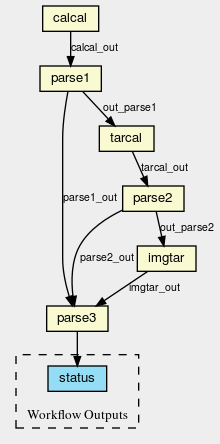
\includegraphics[trim=0 0 0 1cm clip=true,height=.3\textwidth]{cwlgraph}}
    \caption{Prefactor CWL workflow.}
    \label{cwl}
\end{figure}


 After hitting the ``Run Workflow’’ button, an HTTP POST request containing all required information the pipeline is sent to xenon-flow server. Upon reception of the request, xenon-flow will start running the workflow. The configuration of xenon-flow will determine where and how the processes corresponding to the steps will be executed. In our case, xenon-flow is configured to run jobs on the Netherlands ASCI DAS5 cluster located at the VU university using the CWL reference implementation \tit{cwl-runner}. The latter will orderly run all the steps under the control of xenon-flow.

 Upon completion, the concatenated string output is available in xenon-flow and is parsed for successful completion or otherwise. Following successful completion, FITS images produced by the imaging step are available in a specific directory on DAS5, from where the cleaned image (different types are generated) retrieved using the Python \thi{Fabric} module directly into the Django application directory structure. Once on the local machine, the FITS image is converted into an JPEG image for visualisation in the browser using the Python \thi{APLpy} module. An example of images obtained through the developed pipeline is shown in Fig.~\ref{res}.

\begin{figure}[htbp]
    \centerline{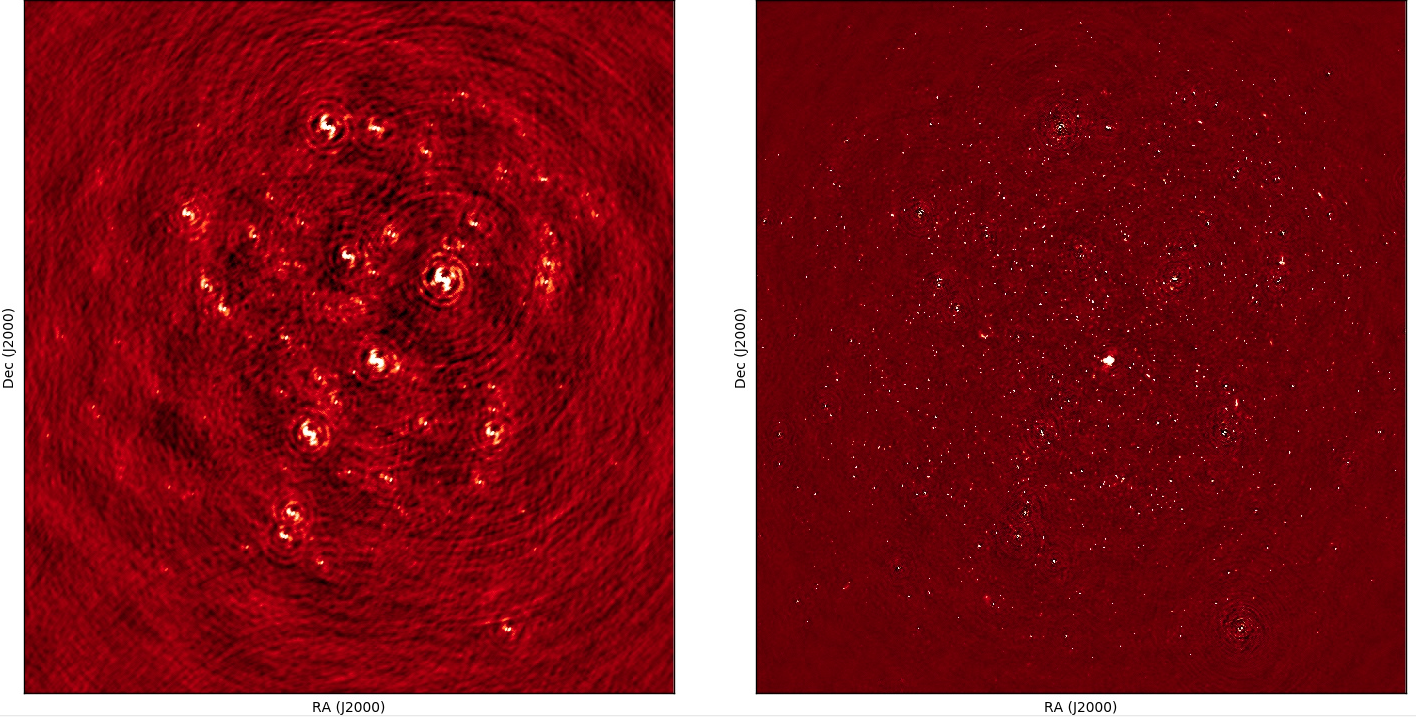
\includegraphics[width=.5\textwidth]{results}}
    \caption{Images of the patch of the sky covered by the processed data. On the left, the uncalibrated data and on the right the DI-calibrated data. DD calibration wil further improve the quality of the image.}
    \label{res}
\end{figure}

\section{Conclusion and future work}

\section*{Acknowledgment}

The preferred spelling of the word ``acknowledgment'' in America is without 
an ``e'' after the ``g''. Avoid the stilted expression ``one of us (R. B. 
G.) thanks $\ldots$''. Instead, try ``R. B. G. thanks$\ldots$''. Put sponsor 
acknowledgments in the unnumbered footnote on the first page.


\bibliographystyle{abbrv}
\bibliography{refs}

\vspace{12pt}
\color{red}
IEEE conference templates contain guidance text for composing and formatting conference papers. Please ensure that all template text is removed from your conference paper prior to submission to the conference. Failure to remove the template text from your paper may result in your paper not being published.

\end{document}
